\chapter{CONTROLLING ATOMIC AND MOLECULAR MODELS}
% !TEX root = hazy1.tex

\section{Atom overview}

The \cdCommand{atom} commands change details of the physical treatment of several
model atoms that are incorporated in the code.

\section{The g-bar approximation}

Many transitions do not have collision rates
(collision rates are for more difficult to determine than radiative rates).
We use various forms of the g-bar approximation to fill in missing data.

The \cdCommand{set gbar} (see page \pageref{sec:Setgbar}) controls aspects
of the g-bar approximation.

\section{Atom FeII [options]}
\label{sec:AtomFeIICommand}

This command adjusts details of the model Fe$^+$ ion.
The default is to
compute the lowest 16 levels, which produce IR emission, as in the real
ion, but to do higher levels, which produce optical and UV emission, using
the simplified and very fast scheme outlined by \citet{Wills1985}
AGN3 describes \feii\ emission in Section 14.5.

When any of the \cdCommand{atom FeII} commands are entered
the Wills et al. scheme is turned off.
A complete model, using 371 levels and described by \citet{Verner1999}, is used instead.
This is far more accurate but also \emph{much} slower.
\citet{Baldwin2004} show some examples of \feii\ spectra of AGN.

\emph{N.B.} the keyword is \cdCommand{FeII}, not \cdCommand{Fe2},
to avoid scanning the number 2 off the command line.
Both \cdCommand{FeII} and \cdCommand{Fe II} (with a space) are accepted.

\subsection{Atom FeII levels}

This changes the number of levels used by the model atom.
The upper
limit is 371 levels and is the default when the large \feii\ model is used.
When the large atom is not used the default is to compute
the lowest 16
levels and treat the remainder of the levels with the \citet{Wills1985}
simple model.
Decreasing the number of levels will speed up the execution
time [roughly proportional to $n^2 \log(n)]$ at the expense of a degraded
simulation of the physics.

\subsection{Atom FeII trace}

This turns on debugging printout for each call to the model atom.

\subsection{Atom FeII redistribution [options]}

The keyword \cdCommand{redistribution} will change
the form of the redistribution
function for various lines within the model atom.

A keyword to specify which set of lines to change is required.
This
is either \cdCommand{resonance} (any line decaying to the ground term)
or \cdCommand{subordinate}
(transitions between excited levels).
The type of redistribution function
to use is also specified.
The options are \cdCommand{PRD} (partial redistribution),
\cdCommand{CRD} (complete redistribution with Doppler core only),
and \cdCommand{CRDW} (complete
redistribution with damping wings).
(The underscore indicates a space.)

The keywords \cdCommand{redistribution show} tells the code to print
the current default redistribution functions.

\subsection{Atom FeII simulate}

This will cause results from the atom to be simulated.  The large model
atom is not actually called.  This is very fast and is a debugging aid.

\subsection{Atom FeII slow}

The keyword \cdCommand{slow} will cause the atom to always be reevaluated.  Normally
the code only reevaluates the atom when the local conditions have changed
significantly.

\subsection{Atom FeII output options}

\feii\ emission is an exercise in uncontrolled complexity.  Hundreds of
thousands of lines contribute to what often appears as a pseudo continuum.
It is not practical to study the list of \feii\ lines
except in a few especially
simple situations such as \hii\ regions.

Three options are available for understanding output from the \feii\ atom.
Most often \feii\ emission is seen as a blended continuum rather than
individual lines.  The general idea is to try to reduce the flood of
information to a manageable level by distilling the emission into what an
observer would actually see.

\emph{\feii\ bands in the main output.}  A series of \feii\ ``bands'' are
automatically entered into the main emission-line output.
Each band represents the total \feii\ emission integrated
over all lines that lie within a range of wavelengths.
This emission appears
in the output with the label ``Fe2b'' and a wavelength close to the center
of the band.
The bands are chosen to represent features that an observer
might be able to measure.

The list of bands is contained in the file
\cdFilename{FeII\_bands.ini}
which is included in the data directory.
This file is intended to be easily changed
by the user.
It explains the format of the information that is needed.
There is no limit to the number of \feii\ bands that can be specified.

\emph{The \cdCommand{save FeII} family of commands}
are described on page \pageref{sec:CommandSaveFeII}
and provide a way to save some predictions.
The following gives an overview of some of these commands.

\cdCommand{save FeII lines}  This reports the intensities
of all emission
lines predicted by the model atom.
The resulting file is very large and
mainly useful for debugging the model atom or understanding where within
the atom a particular feature originates.

\cdCommand{save FeII continuum}  This reports the
total \feii\ emission as a continuous spectrum.
Here a range of wavelengths is broken into a number
of intervals and the total \feii\ emission within each interval is added
together.
The result represents what would be observed by a spectrometer
with a particular resolution and was used to create the plots
in \citet{Baldwin2004}.
Some details, such as the wavelength range and resolution,
are changed with the \cdCommand{set FeII continuum} command
described on page \pageref{sec:CommandSetFeIIContinuum}.

\cdCommand{atom FeII continuum from 1000\AA\ to 7000\AA\  in 1000 cells}
This adjusts the lower and upper bounds and the resolution of the
\feii\ continuum
saved with the \cdCommand{save FeII continuum} command.
The numbers are the lower
and upper limits to the wavelength range in Angstroms and the number of
wavelength cell that occur over this range.

\section{Atom H2 options}

The large model of the \htwo\ molecule, described in \citet{Shaw2005},
will be included if any of the family of \cdCommand{atom H2}
commands appears.
The much
faster three-level model outlined by \citet{Tielens1985a},
\citet{Burton1990}, \citet{Draine1996},
and expanded
by \citet{Elwert2006}, is used by default.
The large molecule is
represented by several thousand levels producing roughly half a million
lines.
AGN3 describes some properties of \htwo\ in section 8.3
and appendix A6.

\emph{NB}  The number ``2'' appears in the keyword for this command.
Any
numerical parameters that appear on the \cdCommand{atom H2}
commands must appear after
this two---the code will check that the first number
parsed off the command line is the number~2.

\subsection{The \cdCommand{set H2} command}

Some details of the physical treatment of the \htwo\ molecule can be
changed with the \cdCommand{set H2} command.

\subsection{\htwo\ output options}

Strong \htwo\ lines will appear in the main emission-line output.
The \cdCommand{save H2} command has many other output options.
The
section in Part 2 of this document describing calling the code as a
subroutine describes several routines that will return predictions of the
large molecule.
The \cdCommand{set line precision} command
will add more significant figures to the wavelengths printed in the main
printout.
This may help isolate a particular line.

\subsection{Atom H2}

With no options, the only effect is to include the large model of the
\htwo\ molecule.

\subsection{Atom H2 chemistry [simple; full]}

This changes how the interactions between the \htwo\ molecule
and the rest of the chemical network are treated.
By default, or if the keyword
\cdCommand{full}
appears, then the fully self-consistent formation and destruction rates
are used when the large \htwo\ molecule is enabled.
If the keyword
\cdCommand{simple} occurs
then expressions from \citet{Tielens1985a} are used instead.

\subsection{Atom H2 collisions [options]}

These commands change various collisional processes within
the \htwo\ molecule.

\cdCommand{atom H2 ortho para collisions on/off}

This turns off
ortho-para changing
collisions with gas particles.

\cdCommand{atom H2 orH2 collisions options}

\cdCommand{atom H2 paH2 collisions options}

These commands determine which of the \htwo\ -- \htwo\ collision data
sets is used.
The default is the \citet{LeeH2H22008} set, which can also
be chosen with the \cdCommand{ORNL} option.
The keyword \cdCommand{Le Bourlet} selects the
\citet{LeBourlot1999} data set.
The keyword \cdCommand{ohH2} adjusts the ortho data and the
keyword \cdCommand{paH2} adjusts the para data set.
One of these keywords must be specified.  Both cannot be adjusted
with the same command.

\cdCommand{atom H2 collisional dissociation on/off}
turns on or off collisional dissociation.
The default is to include it using the estimates given in
\citet{Shaw2005}.
These rates are all only guesses and represent an
uncertainty.

\cdCommand{atom H2 grain collisions on/off} turns off downward
transitions induced by collisions with grains.

By default the code will uses guesses of collisional rate coefficients
using the g-bar method.
Collisional deexcitation for the g-bar transitions
are turned off with the \cdCommand{atom H2 gbar} command.

\subsection{Atom H2 gbar [ off; on]}

The g-bar approximation is a rough relationship between the energy of
a line and its collision rate coefficient.  This can be used to guess a
collisional deexcitation rate coefficient when no real data exist.
This command turns this guess off or on.  It is on by default.

\subsection{Atom H2 levels }

This changes the number of electronic levels within the \htwo\ molecule.
The default is seven and includes the ground and first six bound singlet
electronic states.
This is also the largest number of levels.  At minimum
is three levels, which is sufficient to include the Lyman and Werner bands
in the UV.
This are a necessary minimum number of levels to include the
correct photodissociation processes.
If no number appears but the keyword
\cdCommand{large} does then the code will use the upper limit.

\subsection{Atom H2 limit -4  }

Calculating the level populations and line spectrum of the large \htwo\ molecule is computationally expensive.
The code tries to save time by not
computing the populations when the abundance of \htwo\ is negligible.  This
command changes the limit for the smallest \htwo/H$_{\mathrm{tot}}$ ratio.
The full model
will be computed when the ratio is greater than this limit.
The number
is interpreted as the linear ratio if it is greater than zero and the log
of the ratio if it is less than or equal to zero.
The keyword
\cdCommand{off} turns
off the limit so that the large model of the molecule is always evaluated.
The default limit is 10$^{-8}$, small enough for the large molecule to be
computed across the entire \citet{Tielens1985a} standard PDR
model that is part of the code's test suite.

When the \htwo\ abundance is below this limit the photodissociation,
heating, and cooling rates, are evaluated using expressions in
\citet{Tielens1985a}.
\htwo\ level populations are set to their LTE value so that
self-shielding in the electronic bands is still computed.

\subsection{Atom H2 matrix 43}

Populations of the lower ro-vibration states of the ground electronic
level are determined by two schemes.
The first, and most straightforward,
is the solution of a complete set of balance equations by solving
the system
of balance equations with a master equation approach.
The time needed to solve the linear
algebra increases as a power of the number of levels
so we need to keep
the number of levels as small as possible.
High levels are treated by back
substitution, starting from the highest level with X and proceeding
downwards.
This command sets the total number of levels that are computed
within the matrix.
Levels higher than this will be treated with back
substitution.

If the keyword \cdCommand{off} (note the leading space) or
\cdCommand{none} appears, or if the
number of levels is less than 1, the matrix will not be used.
It the keyword
\cdCommand{all} appears then all levels within X will be done this way.

\subsection{Atom H2 noise [mean, standard deviation, seed]}

This multiplies the rates for collisional processes within the \htwo\ molecule
by a Gaussian random number so that $r' = r\;10^{{\mathrm{rand}}} $.
Here $r$
is the correct rate coefficient and \cdTerm{rand} is an Gaussian
distributed random number.  The first two optional numbers on the command
line set the mean and standard deviation for the Gaussian random numbers.
The first optional number is the mean, with a default of 0.  The second
optional number is the standard deviation with a default of 0.5.  The last
optional number is the seed for the random number generator, which must
be an integer greater than 0.
If the seed is not specified then the system
time is used to generate a random seed.

\subsection{Atom H2 thermal [simple; full]}

This changes how the heating and cooling by the \htwo\ molecule
are treated.
By default, or if the keyword \cdCommand{full} appears,
then the fully self-consistent
heating and cooling rates are used when the large \htwo\ molecule
is enabled.
If the keyword \cdCommand{simple} occurs then expressions
from \citet{Tielens1985a} are used instead.

\subsection{Atom H2 trace [options]}

This turns on trace information concerning the \htwo\ molecule.
The optional
keywords \cdCommand{full}, \cdCommand{iterations},
and \cdCommand{final} will give full information, an overview
of iterations during the convergence, and only final results respectively.
If the keyword \cdCommand{matrix} occurs the code will print
the contents of the matrices
that are used for solution of lower levels within the ground electronic
state.

\subsection{atom H2 output options}

Roughly half a million lines are predicted when the large
\htwo\ molecule is included.
The main emission-line printout includes all significant lines
produced in the ground electronic state but does not include electronic
transitions.
The \cdCommand{print line H2 electronic} command
will include these lines.
The family of \cdCommand{save H2} commands
provides ways to save information such as column densities,
the emission-line spectrum, and details of the effects of \htwo\ on the
conditions in the cloud.

%%%%%%%%%%%%%%%%%%%%%%%%%%%%%%%%%%%%%%%
\section{Atom [H-like \OR{} He-like] [element, options]}
\label{sec:atom_H_He_like}

\subsection{Introduction}
These commands are used to change some details in the treatment of atoms of the
H-like and He-like isoelectronic sequences.\footnote{This was the \cdCommand{hydrogenic}
command in versions 90 and before.}
Atoms of the H-like sequence
have one bound electron and include \hO, He$^{+}$, Li$^{+2}$,
through Zn$^{+29}$.
Atoms of the He-like sequence have two bound electrons and include He$^0$,
Li$^+$, through Zn$^{+28}$.

This implementation of the H-like sequence was initially part of Jason
Ferguson's PhD thesis and is described in \citet{FergusonFerland1997},
\citet{Ferguson2001}, and \citet{BottorffBaldwin2002}.
The physics was expanded
to resolve $nl$ terms by Ryan Porter during a visit to IoA
Cambridge in Fall 2008, as was summarized in 
\citet{LuridianaEtAl09}.
Any number of levels up to $n$ of \nHydroMaxLevel\ can be computed.

The He-like sequence was developed by Ryan Porter as part
of his thesis and it is described in \citet{Bauman2005},
\citet{Porter2005},  \citet{PorterFerland2007}, and
\citet{Porter.R12Improved-He-I-emissivities-in-the-case-B-approximation}.
Ryan Porter unified the two sequences
and expanded the H-like sequence to include all of the physics included
in the He-like sequence.

The two sequences are now unified so the same
\cdCommand{atom AA-like} commands largely work
for both.

The name of one of the iso-sequences must appear on the command line.  
The options are \cdCommand{H-like} and \cdCommand{H-like}.
Only one iso-sequence can be modified
with a single command.
By default all ions of the iso-sequence are modified.
If the keyword \cdCommand{element} and
the name of an element appears then
only that ion is modified.  
The following are some examples

\begin{verbatim}
# only change hydrogen itself
atom H-like element hydrogen levels 8
# change the entire He-like sequence
atom He-like levels 9
\end{verbatim}

\subsection{Structure of the model atoms}

The model atoms include a certain number of resolved and collapsed levels
as shown in Figure \ref{fig:LevelsResolvedCollapsed}.
The lower $n_{resolved}$ levels are $nl$ resolved.
Another $n_{collapsed}$ levels,
which replace the $nl$ terms with an $n$ configuration,
are above the resolved levels.

\begin{figure}
\centering
\includegraphics[scale=0.7]{LevelsResolvedCollapsed}
\caption[Resolved and collapsed levels]
{\label{fig:LevelsResolvedCollapsed}This shows  
resolved and collapsed levels for a typical H- or He-like species.
The set of horizontal bars on the left are energy levels with
principal quantum numbers ranging from 1 to 7, increasing from bottom to top.
The lowest three configurations are resolved into $nl$ terms while
higher shells are treated as collapsed levels, in which the $nl$ terms
are assumed to be populated according to their statistical weight.
The levels are adjusted with the \cdCommand{atom AA-like levels} command.
This is a cartoon and does not represent any particular species.}
\end{figure}

The physics of the resolved levels is exact while that of the
collapsed levels is more approximate since the entire \emph{n} configuration is
treated as a single level assuming that the $nl$ terms within the \emph{n} configuration 
are populated according to statistical weight.
This is a good assumption at high densities, as
shown by \citet{PengellySeaton1964}.

The total recombination coefficient is the sum to over all possible bound levels.
The model has a finite, often small, number of levels. 
Recombination coefficients to each level are derived from the photoionization cross
section using the Milne relation (AGN3).
The recombination to these levels is less than the total.
We ``topoff'' the model by adding the remaining recombination coefficient
to the model atom, as controlled with the
\cdCommand {atom xx-like topoff} command.

By default only lines produced by resolved levels
are included in the printout.
The \cdCommand{print line iso collapsed} command,
described on \pageref{sec:CommandPrintLineIsoCollapsed},
will cause lines produced by the collapsed
levels to be included in the printout.
See the discussion of 
the \cdCommand{print line iso collapsed} command for more details.

\subsubsection{The H-like sequence}
Figure \ref{fig:LevelsResolvedCollapsed} shows an H-like system.
Resolved configurations are split into $nl$ levels.
Collapsed levels each represent one principal quantum number.
By default there are 10 resolved and 15 collapsed levels for H$^0$ and He$^+$,
and 5 resolved and 15 collapsed levels for heavier elements.

The H-like iso sequence models atoms can extend up to any principle
quantum number between the limits $4 < n \le \nHydroMaxLevel$.
The size is limited mainly
by the available memory and computer time.
Increasing the
number of levels allows a better representation of the collision physics
that occurs within higher levels of the atom at the expense of longer
execution times and greater memory requirements.

\subsubsection{The He-like sequence}

The model atom resolves $n$-levels into $nLS$ levels,
and the 2 $^3P$ term is split into three $nLSJ$ levels.
For a given maximum principal quantum number
$n_{\max}$, there will be a total of $n_{\max}^2 + n_{\max} +1 nLS$ levels.  
The default number of resolved levels for He$^0$ is 6, resulting in
43 $nLS$ levels, 
there are five resolved levels
for C, N, O, Fe, and Zn, and three resolved levels
for all remaining elements.
Increasing $n_{\max}$ allows a better representation of the atom's
emission,
especially the collision physics that occurs within higher levels
of the atom,
but at the expense of longer execution times and greater memory
requirements.

There are also 20 collapsed levels for He$^0$ and one collapsed level for heavier elements.
These collapsed levels
bring together all of the individual $nLS$ terms as one pseudo-level.
The
recombination coefficient into this pseudo-level is the sum of recombination
coefficients into the individual terms plus the recombination topoff.
Transition probabilities from this pseudo-level are calculated as follows.
\begin{equation}
A(n_u \to n_lL_lS)= \frac{\sum_{L_u=L_pm 1} g_{L_{u}S} A(n_uL_uS\to
n_lL_lS)}{\sum_{L_u=L_l\pm 1}}.%49
\end{equation}
This causes the collapsed level to behave exactly as if it were a set of
resolved terms populated according to statistical weight.

There is no limit to the number of levels other than computational resources
like memory and time.

\subsection{Atom H-like collisions\dots }

Collisional processes, both between levels ionization, are turned off
with this command.  They are all on by default.  This command is mainly
used for debugging.  Separate collisional processes can be turned off with
the following options.  Only one option is recognized per command line so
multiple commands are needed to turn off several processes.  If no
sub-options are recognized then all collisional processes are disabled.
This command turns off collisions for all elements along the H-like
isoelectronic sequence.

\cdCommand{atom H-like collisions l-mixing off}\footnote{This was the 2s2p option in versions 94 and before.  The 2s2p option
still exists for backward compatibility.}
This turns off \emph{l}-mixing $2s-2p$ collisions.

\cdCommand{atom H-like collisional ionization off}
This command turns off collisional
ionization by thermal electrons of all levels.
Ionization by
cosmic rays is not affected by this command.

\cdCommand{atom H-like collisional excitation off}
This command turns off collisional
excitation of all levels, except for 2s-2p.

\cdCommand{atom H-like collisions off}
All three collisional processes will be turned
off if none of the three keywords are recognized.

\emph{Warning!}  The code will require a very number of zones
if collisions
are turned off in an optically thick cloud with a large
$(n \gg 15)$ hydrogen atom.
Collisions will normally hold populations of very highly excited
levels to values very near LTE.
The FIR and radio lines will have very
small line optical depths due to the correction for stimulated emission.
When collisions are absent, the normal tendency of departure coefficients
to increase with principal quantum number means that FIR and radio lines
will strongly mase.
The code dynamically adjusts the zoning to prevent
these maser optical depths from diverging to minus infinity.
A very large
number of zones will be required to spatially resolve the masing region.
This is a totally artificial, not physical, effect.
The solution is to
not turn off collisions with a large atom when performing a
simulation with more than a trivial thickness.

\subsection{Atom He-like collisions \dots.}

Collisional processes between levels and collisional ionization are turned
off with this command.
Separate collisional processes can be turned off
with the following options.
Only one option is recognized per command line
so multiple commands are needed to turn off several processes.
If no
sub-options are recognized then all collisional processes are disabled.
This command turns off collisions for all elements along the He-like
isoelectronic sequence.

\cdCommand{atom He-like collisions l-mixing off}  This command
turns off all
collisions within the same $n$ level for all elements in the helium-like
isoelectronic sequence.
Both $L$- and $S$-changing collisions are turned off.

\cdCommand{atom He-like collisions l-mixing Pengelly [Vrinceanu]}  This
changes to the \citet{PengellySeaton1964} formalism rather than
currently the default,
based on \citet{Vrinceanu2001} for $L > 2$.

\cdCommand{atom He-like collisions l-mixing thermal [ averaging, no averaging]}
The \cdCommand{no thermal averaging} option calculates the
\citet{Vrinceanu2001}
collision strengths at an impact energy equal to $kT$,
rather than averaging
over a Maxwellian distribution.
This is the default when a small atom is
used.
Thermally averaged collision strengths are used when the atom is
large.

\cdCommand{atom He-like collisions excitation}  This command
turns off collisional
excitation, for all $n_u \not= n_l$ transitions,
for all elements in the helium-like
isoelectronic sequence.

\cdCommand{atom H-like collisional ionization off}
This command turns off collisional
ionization by thermal electrons of all levels.

\subsection{Atom [H-like \OR{} He-like]  continuum lowering off }
This command disables continuum lowering processes due to particle packing,
Debye shielding, or Stark broadening.  The processes are active by default
and implemented following \citet{Bautista00}.  This command applies
to the entire isoelectronic sequence.

\subsection{Atom [H-like] damping off}

Rayleigh scattering, continuum scattering due to the extreme damping
wings of hydrogen Lyman lines, is turned off with the \cdCommand{damping off} option.
\hi\  Rayleigh scattering is a significant opacity source in clouds that have
large column densities of neutral material
($N$(\hO $) > 10^{23} \mathrm{cm}^{-2}$).

This only disables \hi\ Rayleigh scattering.  
The \cdCommand{He-like} option is not supported. 

\subsection{Atom He-like dielectronic recombination [off] }

This option turns dielectronic recombination off for the entire
isoelectronic sequence.
Dielectronic recombination is included by default.
This command only turns off DR.
It affects all elements of the He-like iso sequence.

\subsection{Atom [h-like \OR{} he-like] error generation}

Monte Carlo error analysis can be performed with this command.
Randomly
generated Gaussian errors are applied to atomic data.
The parameter X is
an integer used to set the seed of the random number generator.

The pessimistic option will choose the largest of two standard deviations
for each piece of atomic data.
The full command would look something like
\begin{verbatim}
atom he-like error generation pessimistic 5
\end{verbatim}
where the number is the seed for the random number generator. Without the
pessimistic keyword the default optimistic values are used.

\subsection{Atom He-like FSM}

For $L > 2$, levels with the same $n$ and $L$ but different $S$ are strongly
mixed due to the spin-other-orbit interaction.
This option modifies transition probabilities to account for this fine-structure mixing.
The effect on multiplet emissions is not large.
See \citet{Bauman2005} for a discussion and calculation of this effect 
in a zero-density $J$-resolved helium atom.

\subsection{Atom He-like gbar options}

The code employs various forms of the $\bar g$
approximation to fill in collision strengths for those transitions with
no quantal calculations.
This command changes which approximation is used.
The options are \cdCommand{Vriens} for the \citet{Vriens1980} and
\cdCommand{off} to set this to zero.
This only exists for the He-like iso sequence.

\subsection{Atom [h-like \OR{} he-like] levels options}

This set of commands controls the model atomic structure shown in 
Figure \ref{fig:LevelsResolvedCollapsed}.

The number of levels can only be set once at the very start of a
calculation when space is allocated for the hydrogenic arrays.
If the code
is used to run a grid of models then only the first occurrence of
\cdCommand{atom xx-like levels} is honored and all following occurrences
are ignored.

\subsubsection{Atom He-like [resolved, collapsed] levels 4 [element iron]}

One of the keywords \cdCommand{resolved} or \cdCommand{collapsed} must appear.
This sets the number of resolved or collapsed levels.
The argument gives the principal quantum
number $n$ for the number of levels.
In the case of collapsed levels the number of added levels will be equal to the argument.
In the case of resolved levels a large number of resolved terms may be needed
to produce the requested number of principal quantum numbers.

The following sets most iso sequence models to a small number of levels
but does a high quality simulation of theH- and He- like Fe ions.
\begin{verbatim}
% most ions have small models
atom H-like levels small
atom He-like levels small
% resolve the lowest n=10 shells, these take well more than 10 levels
atom H-like levels element iron resolved levels 10
atom He-like levels element iron resolved levels 10
% 15 collapsed levels on top
atom H-like levels element iron collapsed levels 15
atom He-like levels element iron collapsed levels 15
\end{verbatim}

\subsubsection{Atom [h-like \OR{} he-like] levels LTE}

This will set the level populations to their LTE values.

\subsubsection{Atom [h-like \OR{} he-like] levels print}

This produces a summary of the number of levels for all ions of the iso sequences.
It reports the highest principal quantum number of the resolved levels,
the number of $nls$ terms in these $n$ configurations,
and the number of collapsed levels.

\subsubsection{Setting the number of levels with keywords}

If no numbers occur then we look for a keyword to specify preset sizes.
The code will use the smaller of either the preset size or the current size.

\emph{The H-like iso sequence.}

The keyword
\cdCommand{large} or \cdCommand{small}
specifies either 40 or 5 resolved levels.
Ten collapsed levels are used for the \cdCommand{small} option.

The following would set the full H-like isoelectronic
sequence to a small number of levels, then reset hydrogen, helium,
and iron to a large number.
\begin{verbatim}
atom H-like levels small
atom H-like levels large element hydrogen
atom H-like levels large element helium
atom H-like levels large element iron
\end{verbatim}

\emph{The He-like iso sequence.}
If no number appears on the command, but the keyword \cdCommand{large} or
\cdCommand{small} does,
then the number of levels will be large enough to extend
to either $n = 40$ or 3.
Actually, the atoms are
coded so that there is no limit to the number of levels that
can be included, other than the memory and computer time requirements.

Use the \cdCommand{atom xx-like print} to confirm that you are using
the expected number of levels.

\emph{Warning!}  Note that the command
\begin{verbatim}
atom H-like levels large
\end{verbatim}
will set all \LIMELM\ hydrogenic atoms to a large number of levels.
This would
require roughly half a gigabyte of memory for the H-like sequence along,
and would be very slow on today's computers.
It is best to set only the
most important elements to large levels.

\subsection{Atom [H-like \OR{} He-like] Lyman options}

This set of commands changes the treatment of the Lyman lines.
For this purpose, the Lyman lines are all resonance lines,
lines whose lower level is the ground state,  of the  iso sequences.
(Actually, only the \hi\ resonance lines are Lyman lines.)

\subsubsection{Atom [H-like \OR{} He-like]  Lyman extra 1000}  

Atoms and ions of the H-like and He-like
isoelectronic sequences use complete multi-level model atoms.
The number of levels included is limited mainly by processor speed and
available memory.
Higher Lyman lines (used here to mean permitted lines that connect directly
to ground) have little impact on emission since they
scatter and are degraded
into Balmer lines and L$\alpha $.
However, an absorption spectrum will show them
as a series of lines converging onto the photoionization continuum from
the ground state.
The code includes a large number of ``extra'' Lyman lines,
included as absorbers with optical depths output with
the \cdCommand{save line optical depth} command,
but not treated as part of the multi-level atoms.
The default number of higher Lyman lines is 100, and
this can be changed to any number with this command.

This changes the number of extra levels for the entire iso-electronic sequence.

\subsubsection{Atom H-like Lyman pump}  

These commands control how continuum fluorescent excitation, ``line pumping'', is treated.
They only modify the treatment of \hi\ so the \cdCommand{H-like} keyword must appear.

\subsubsection{Atom H-like Lyman pumping off}  
This turns off continuum radiative pumping of the Lyman lines of \hi.
This is one way to take into account the possible
presence of Lyman absorption lines in the incident continuum.

\subsubsection{Atom H-like Lyman pumping scale 3}
The continuum radiative pumping rate
of the Lyman lines of \hi\ will be multiplied by the scale factor
that appears on the line.
This is meant to take into account the possible presence of
Lyman lines in emission or absorption in the incident continuum.
The pumping
rate is normally set by the intensity of the coarse continuum at the line
wavelength.
The number that appears on the command line is a scale factor
that multiplies this continuum.\footnote{In versions C08 and before a value of 0 would produce black Lyman lines.
Starting in C10 values $\le 0$ are interpreted as logs
so a value of 0 will result in a scale factor of unity.}
Numbers $\le 0$ are interpreted as a log and
the \cdCommand{log} keyword will force interpretation as a log.
A value of greater than 1 would correspond to Lyman lines
in emission in the incident radiation field.
A scale factor of 
2 would simulate the presence of stellar Lyman emission lines with peak
intensities twice those of the neighboring continuum.

\subsection{Atom [h-like \OR{} he-like] NO RECOmbination INTErp}

The code normally derives recombination coefficients by interpolating
on a table that lives in the data directory.
This command tells the code
to compute recombination coefficients on the fly by integrating over the
photoionization cross section.

\subsection{Atom [h-like \OR{} he-like] REDI}

There are three options, PRD, CRD, and CRDW, representing partial
redistribution, complete redistribution (doppler core only, no wings)
and complete with wings, respectively.  Additional options are ALPH
(to set value for Lyman $\alpha$), RESO (to set value for other
resonance lines), and SUBO (to set value for subordinate lines).  SHOW
to prints diagnostic output to confirm selected options.

\subsection{Atom [h-like \OR{} he-like]  redistribution [options]}

This changes the form of the redistribution
function for various lines within the model atom.
This command is only
used if you are not happy with the default redistribution functions.
The command changes the redistribution functions for entire iso-sequences.

A keyword to specify which set of lines to change is required.
This is one of \cdCommand{alpha} (the H-like $2p - 1s$ transition or the He-like
$2\, ^1P - 1\, ^1S$ transition)), \cdCommand{resonance} (any higher Lyman line
decaying to the ground term), or \cdCommand{subordinate}
(all Balmer, Paschen, etc lines).
The type of redistribution function to use must also be specified.
The options are \cdCommand{PRD} (partial redistribution), \cdCommand{CRD} (complete redistribution
with Doppler core only), and \cdCommand{CRDW}
(complete redistribution with damping wings).
(The underscore indicates a space.)

The keyword \cdCommand{show} prints the current default
redistribution functions at the time when the command is parsed.

There is at present a fundamental uncertainty in the computation of the
line radiation pressure for transitions such as L$\alpha $.
For a simple two-level
atom with incomplete redistribution, it has long been known that the
line-width is proportional to ($a\tau)^{1/3}$
(\citealp{Adams1972}, \citealp{Harrington1973}; $a$ is
the damping constant).  It is also easily shown that for complete
redistribution and a frequency independent source function that the line
width would be determined by inverting the Voigt function, and hence
proportional to ($a\tau)^{1/2}$.
Line interlocking, whereby scattered Balmer line
radiation broadens the upper level of L$\alpha$
(\citealp{Hubbard1985}), can
alter the line width, as can collisional effects when the density is high
enough for distant collisions to broaden the line.
These effects cause
major differences in radiation pressure and emergent flux (factors of
several) for \la, which can easily have an optical depth of
$10^7$--$10^9$, when
Balmer lines are also optically thick.  T
his command determines which
approximation is used.
The default condition is incomplete redistribution,
which minimizes the line width and radiation pressure.  This issue is
discussed further in \citet{Elitzur1986}.

\subsection{Atom [h-like \OR{} he-like] topoff off} 

This turns top off off or on.
The default is to be on and the keyword \cdCommand{off} disables topoff.
Topoff is necessary to obtain the correct total
radiative recombination rate coefficient with a finite number of levels.
Because only a finite number of levels can be computed the sum
of the total
recombination coefficient will be less than the sum to infinity.
This difference must be added somewhere to conserve the
total recombination rate.  
This changes the entire iso-sequence.

%%%%%%%%%%%%%%%%%%%%%%%%%%%%%%%%%%%%%%%%%%%%%%
\section{Atom Chianti [ options ]}
\label{sec:SetChianti}

This controls the use of the 
\href{http://www.chiantidatabase.org/}{Chianti} database 
(\cite{Dere.K97CHIANTI---an-atomic-database-for-emission}; \cite{Landi2012}).
The \cdCommand{save chianti} command described on 
page \pageref{sec:CommandSaveChianti} can be used to export parts of 
the Chianti data.

The Chianti database does not contain collision strengths for subordinate transitions.
By default, \Cloudy\ will use the gbar approximation to estimate collision strengths for allowed transitions that do not have data. 
The \cdCommand{Set Gbar} command controls the use of gbar in Chianti and is described on page \pageref{sec:Setgbar}.

\subsection{Atom Chianti \cdFilename{"masterlist.ini"}}
By default, \Cloudy\ uses selected Chianti species between phosphorus and zinc, 
specifically including Fe VI through Fe XXIV.
These species are listed in the \cdFilename{CloudyChianti.ini} masterlist file in the 
\cdFilename{data/chianti/masterlist} directory.
Files in that directory give other sets of species.

If a double quote appears on the line then the filename
between the pair of double quotes will be used instead of
the \cdFilename{CloudyChianti.ini} file.
This makes it possible to create masterlist files that select portions
of Chianti.
The code will search for the masterlist file in the current directory then in
\cdFilename{data/chianti/masterlist}.

\subsection{Atom Chianti off} 
will disable all of Chianti.

\subsection{Atom Chianti hybrid} 
Hybrid, the merging of the Chianti data with the Opacity Project data, 
is on by default if Chianti is on.
The \cdCommand{no hybrid} option disables the Opacity Project data and only uses Chianti.

\subsection{Atom Chianti print} 
will print which Chianti ions are being used
along with the number of levels.
 
\subsection{Atom Chianti Levels} 
sets the maximum number of Chianti energy levels. 
Some ions have a very large number of levels.
These have a significant impact
on the execution time but produce only weak lines and have a minor effect
on the cooling for photoionized clouds.
By default we limit the number of energy levels for Chianti iron species to 
\nChiantiPhotoLevelsFe\ and all other elements to \nChiantiPhotoLevels.
Plasmas in collisional equilibrium tend to be hotter, for a given
stage of ionization, than a photoionized plasma.  
The \cdCommand{Coronal} command, described on
page \pageref{sec:CommandCoronalEquilibrium}, is used for
the collisional ionization case.
The limits to the number of levels are then \nChiantiCollLevelsFe\ for iron 
and \nChiantiCollLevels\ for all others.
The \cdCommand{levels} option will overwrite these limits.
The first number, i, is the iron level limit, while the second number, 
j, is for all other Chianti elements.
If no numbers appear but the keyword \cdCommand{MAX} does, we use all 
of the available energy levels.

\subsection{Atom Chianti [experimental theoretical]}
By default we use experimental Chianti energies.
The \cdCommand{theoretical} option causes \Cloudy\ to only use theoretical 
energies.
This provides significantly more levels and transitions, 
however the error in wavelength is larger.

The \cdCommand{atom Lamda} command, described on page \pageref{sec:SetLamda},
and the \cdCommand{atom Stout} command, described on page \pageref{sec:SetStout},
do similar work for the Lamda and Stout databases.

\section{Atom Lamda [ON , OFF]}
\label{sec:SetLamda}
This enables or disables molecular models from Lamda, the Leiden Atomic and Molecular
Database ( http://www.strw.leidenuniv.nl/~moldata/ , 
\citet{Schoier.F05An-atomic-and-molecular-database-for-analysis}).   
Note that some molecules in LAMDA are not
currently known to \Cloudy 's chemistry.  \Cloudy\ therefore has no means by
which to predict the abundance of those molecules.  In such cases, the
LAMDA models are simply ignored. 

The \cdCommand{atom  Chianti} command, described on page \pageref{sec:SetChianti},
and the \cdCommand{atom  Stout} command, described on page \pageref{sec:SetStout},
do similar work for the Chianti and Stout databases.


\section{Atom Stout [on , off, no hybrid][print][levels \{j, MAX\}]}
\label{sec:SetStout}
The command controls the use of the Stout database.

\subsection{Atom Stout [on off]} 
command will enable or disable the use of the Stout database.
It is on by default.

\subsection{Atom Stout \cdFilename{"masterlist.ini"}}
The species included in the filename between quotes will be used.
By default we use species listed in the \cdFilename{Stout.ini} file in the 
\cdFilename{data/stout/masterlist} directory.
This makes it possible to create \cdFilename{ini} files that select portions of Stout.
The code will search for the masterlist file in the current directory then in
\cdFilename{data/stout/masterlist}.

\subsection{Atom Stout hybrid} 
Hybrid, the merging of the Stout data with the Opacity Project data, 
is on by default.
The \cdCommand{no hybrid} option disables the Opacity Project data 
and only uses Stout.

\subsection{Atom Stout print} 
will print which Stout species are being used
along with the number of levels.

\subsection{Atom Stout Levels} 
This sets the maximum number of Stout energy levels. 
Some ions may have a very large number of levels.
These have a significant impact on the execution time but produce only weak lines and have a minor effect
on the cooling for photoionized clouds.
By default we limit the number of energy levels for Stout species to 100.
The \cdCommand{levels} option will overwrite the limit.
A number following the \cdCommand{levels}, j, will limit the number of Stout levels to that number.
If no numbers appear but the keyword \cdCommand{MAX} does, we use all 
of the available energy levels.

The \cdCommand{atom Chianti} command, described on page \pageref{sec:SetChianti},
and the \cdCommand{atom Lamda} command, described on page \pageref{sec:SetLamda},
do similar work for the Chianti and Lamda databases.

